\documentclass{article}
\usepackage{amsmath}
\usepackage{graphicx}
\graphicspath{ {images/} }
\usepackage[inline]{enumitem}  
\usepackage[letterpaper, total={7.5in, 10in}]{geometry}
\title{Spy Problem 4}
\author{Andrew Shen, Kevin Yang, Richard Ye, and Daniel Zhan}
\begin{document}
	\maketitle
	\section{Problem}
	(Sweet Revenge is close at hand!!) The spy has tracked Eco Li and is ready to pay him back for killing his buddy, Sal Manella. The spy is in a Cartesian (air) plane flying at $10,000\;ft$ when he spots the cave of h is nemesis. There is no place to land, so decides to para(bola?)chute into Li's domain. In order to controol where he lands, he freefalls (is this a Six Flags ride?) for a whlie before opening his parachute. He realizes that, to land safely, he must meet two criteria:
	\begin{enumerate}
		\item[a)] he must open the chute at an altitude of about $1500\;ft$ (to pick the safest spot)
		\item[b)]the total descent cannot exceed 2 minutes (otherwise Li will spot him and he could experience the same fate as poor Sal Manella)
	\end{enumerate}
	\textbf{Does our hero land safely?}
	\\
	Note: the weight of the spy is $W = mg= 175\;lb$, gravitational acceleration is $g=32\;\frac{ft}{s^2}$, and the constants of air resistance are $k=0.003$ during freefall and $k=0.56$ during the chute portion.\\
	At minimum, your solution should list the initial conditions for each phase, the solution functions for the velocity and the distance fallen for each phase; tell how long (nearest second) he should free fall before opening the chute and the distance fallen at that time, the total elapsed time the descent took place.
	\section{Solution}
	\subsection{Setting Up the Solution}
	For the convenience of the problem, let us define the upwards direction as positive and the downwards direction as negative. Thus, the force of gravity, along with the gravitational acceleration and velocity of the object, is negative. On the other hand, the resistive force is positive.
	\subsection{Modeling the Problem}
	To model the problem, we examine the forces upon the spy: the downwards force of gravity and the upwards force of air resistance. Thus,
	\begin{center}
		$F=ma=m\left(\frac{dv}{dt}\right) = -W + kv^2$
	\end{center}
	After some algebraic manipulation to turn the model into a first order homogenous seperable differential equation, we get:
	\begin{center}
	$m\left(\frac{dv}{dt}\right) = -W 
	+ kv^2$ \\
	$\rightarrow \frac{dv}{dt} = g-\frac{k}{m}v^2$ \\
	$\rightarrow \frac{dv}{dt} = g(\frac{k}{mg}v^2 - 1)$\\
	Let us define $a^2 = \frac{k}{mg}$\\
	$\rightarrow \frac{dv}{dt} = g(a^2v^2 - 1)$
	\end{center}
	\subsection{Solving the Differential Equation}
	\begin{center}
	$\rightarrow \frac{dv}{dt} = g(a^2v^2 - 1)$ \\
	$\rightarrow \frac{dv}{a^2v^2 - 1} = gdt$ \\
	$\rightarrow \int \frac{dv}{a^2v^2 - 1} = \int gdt$ \\
	We apply partial fraction decomposition.\\
	$\rightarrow \int \frac{-1}{2}\frac{1}{av+1}+\frac{1}{2}\frac{1}{av-1} dv= \int gdt$\\
	$\rightarrow \frac{-1}{2a}ln(av+1)+\frac{1}{2a}ln(av-1) = gt+C_1$\\
	$\rightarrow \frac{1}{2a}ln\left(\frac{av-1}{av+1}\right)$ \\
	$\rightarrow$
	$\begin{cases}
		\frac{-1}{a}tanh^{-1}(av) & |v| \le \frac{1}{a} \\
		\frac{-1}{a}coth^-1(av) &|v| <  \frac{1}{a}
	\end{cases}$
	$=gt+C$\\
	$\rightarrow v=$
	$\begin{cases}
			\frac{1}{a} tanh(-agt+C) & |v|\le \frac{1}{a} \\
			\frac{1}{a} coth(-agt+C) &|v| >  \frac{1}{a}
		\end{cases}$
	\end{center}
	\subsection{Solving the First Portion of Descent}
	In the first portion of descent, the spy is in freefall so $k = 0.003$. Thus, $a_1 = \sqrt{\frac{k}{mg}} = \sqrt{\frac{0.003}{175}} \approx 0.00414$. In this portion, the initial velocity $v_{1_0} = 0$ and $x_{1_0} = 10000$. 
	\subsubsection{Solving for the Velocity Function}
	We can easily tell that in this portion, the velocity cannot exceed $\frac{1}{a_1^2}$. Thus, the equation that models this portion of descent is,
	\begin{center}
		$v_1(t)=\frac{1}{a_1} tanh(-a_1gt+C_1)$
	\end{center}
	We substitute in the initial condition of $v_{1_0} =0$ to find,
	\begin{center}
	$v_1(0) = 0 =\frac{1}{a_1} tanh(-a_1g*0+C_1)$ \\
	$\rightarrow C_1 = 0$
	\end{center}
	Now we have, 
	\begin{center}
		$v_1(t)=\frac{1}{a_1} tanh(-a_1gt)$
	\end{center}
	\subsubsection{Solving for the Distance Function}
	Since we have the velocity function, we can find the distance function easily.
	\begin{center}
		$v_1(t)=\frac{dv}{dt} =\frac{1}{a_1} tanh(-a_1gt)$\\
		$\rightarrow dv = \frac{1}{a_1} tanh(-a_1gt)dt$\\
		$\rightarrow \int dv = \int \frac{1}{a_1} tanh(-a_1gt)dt$\\
		$x_1(t) = \frac{1}{2a_1g} ln(cosh(-a_1gt))+C_2$
	\end{center}
	We substitute in the initial condition of $x_{1_0} =10000$ to find,
	\begin{center}
	$x_1(0) = 10000 = \frac{1}{2a_1g} ln(cosh(-a_1gt))+C_2$\\
	$\rightarrow C_2 = 10000$
	\end{center}
	Now we have,
	\begin{center}
	$x_1(t) = \frac{1}{2a_1g} ln(cosh(-a_1gt))+10000$
	\end{center}
	%\subsubsection{Solving for Time to Release Parachute}
	%We know that the spy wishes to release his parachute at around $1500\;ft$ so we simply use a calculator to solve,
	%\begin{center}
	%$x_1(t) = 1500 \frac{1}{2a_1g} ln(cosh(-a_1gt))+C_2$ \\
	%$\rightarrow t = 40.424768 \approx 40\;s$
	%\end{center}
	%At this time, the spy's velocity is $v_1(40) \approx -241.510934\;
	%\frac{ft}{s}$ and the spy's distance to the ground is $x_1(40) \approx 1602.586271\;ft$ so the spy has fallen $10000-1602.586271 = 8397.413729\;ft$ in $40\;s$.
	\subsection{Solving the Second Portion of Descent}
	In the second portion of descent, the spy is in freefall so $k = 0.56$. Thus, $a_2 = \sqrt{\frac{k}{mg}} = \sqrt{\frac{0.56}{175}} \approx 0.05657$.%In this part of the ascent, we enter with intial conditions of $v_{2_0} = -241.510934\;\frac{ft}{s}$ and $x_{2_0} = 1602.586271\;ft$. 
	\subsubsection{Solving for the Velocity Function}
	We can easily tell that in this portion, the velocity has already exceeded $\frac{1}{a_2^2}$. Thus, the equation that models this portion of descent is,
	\begin{center}
		$v_2(t)=\frac{1}{a_2} coth(-a_2gt+C_3)$
	\end{center}
	%We substitute in the initial condition of $v_{2_0} =-241.510934$ to find,
	%\begin{center}
	%$v_2(0) = 0 =\frac{1}{a_2} tanh(-a_2g*0+C_3)$ \\
	%$\rightarrow C_3 \approx 0.0733272973$
	%\end{center}
	%Now we have, 
	%\begin{center}
	%	$v_2(t)=\frac{1}{a_2} tanh(-a_2gt+C_3)$
	%\end{center}
	\subsubsection{Solving for the Distance Function}
	Since we have the velocity function, we can find the distance function easily.
	\begin{center}
		$v_2(t)=\frac{dv}{dt} =\frac{1}{a_2} tanh(-a_2gt+C_3)$\\
		$\rightarrow dv = \frac{1}{a_2} tanh(-a_2gt+C_3)dt$\\
		$\rightarrow \int dv = \int \frac{1}{a_2} tanh(-a_2gt+C_3)dt$\\
		$x_2(t) = \frac{1}{2a_2g} ln(cosh(-a_2gt+C_3))+C_4$
	\end{center}
	%We substitute in the initial condition of $x_{2_0} =1602.586271$ to find,
	%\begin{center}
	%$x_2(0) = 1602.586271 = \frac{1}{2a_2g} ln(cosh(-a_2gt+C_3))+C_4$\\
	%$\rightarrow C_4 \approx 1577.079$
	%\end{center}
	%Now we have,
	%\begin{center}
	%$x_2(t) = \frac{1}{2a_2g} ln(cosh(-a_2gt+C_3))+1577.079$
	%\end{center}
	\subsubsection{Solving for the Time to the Ground}
	Since we do not know the actual location to release the parachute, it is best to use trial and error to find the correct height. To do so, I have created an excel spreadsheet that calculates the two times of descent and I tested values until I got an answer as close to $120\;s$ as possible but not exceeding it. \\
	Every value is calculated using the above derived functions or their inverse function. The derivation is just subtituting in numbers into the above functions and their inverses again and again.\\
	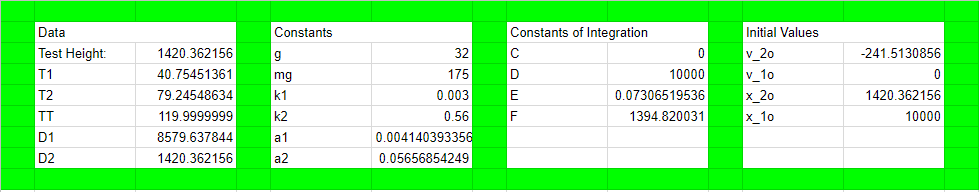
\includegraphics[scale=0.75]{images/p6tne.PNG}
	$Test\; height$ is simply an independent variable that I changed to test for the correct height. $T1$ is the time taken during the first portion of descent and $T2$ for the second portion. $D1$ is the distance traveled in the first portion and $D2$ is the distance traveled in the second portion. The constants are the constants provided and the constants are integration are $C_1,\; C_2,\; C_3,\; C_4$ respectively from top to bottom. The initial conditions for each state is also clearly listed.\\
	The time the spy takes to reach the ground will be approximately $120\;s$.
	\subsection{Final Remarks}
	As you can see, if the spy releases his parachute at $1420\;ft$ from the ground, he will successfully make it to the ground within $2\;min$. In fact, the spy will reach the ground at approximately $120\;s$. Although $1420\;ft$ isn't neccessarily close to $1500\;ft$, it is the first height he can survive at so the spy has to be on it being close enough.
\end{document}